\documentclass[12pt]{article}

\usepackage{ceai}
\graphicspath{{../figs/}}

\begin{document}
\doublespacing

\title{CE 488/5588: Applied AI for Engineering\\ \large Topic 15: Introduction to Large Language Models}
\author{}
\date{}
\maketitle

\begin{ch-box}
This chapter begins a new part of the course. Earlier topics focused on machine learning and deep learning as predictive or generative tools. We now turn to language-centered foundation models. The motivation is not only that modern large language models (LLMs) are impressive, but that engineering work is already organized around language-like artifacts: design codes, specifications, reports, spreadsheets, calculation sheets, tables, plots, CAD notes, emails, and source code. If these materials can be searched, summarized, connected, and reasoned over faster, then analysis and design may be accelerated even when they are not fully automated.
\end{ch-box}

\section{Why This Topic Matters for Engineers}

Much of modern engineering is document-heavy. Before a design is finalized, an engineer may need to read standards, compare alternatives, inspect previous reports, interpret tables, examine calculations, and coordinate across software tools. In practice, this means that engineering knowledge is often stored in semi-structured text long before it becomes a final number or drawing.

LLMs matter because they operate directly on this kind of material. They do not replace mechanics, physics, or engineering judgment. Instead, they provide a new interface for interacting with technical knowledge. A well-designed workflow can help an engineer:

\begin{itemize}
    \item search large bodies of technical documents in natural language;
    \item summarize long reports or standards before deeper review;
    \item compare alternative design assumptions across multiple sources;
    \item draft code, scripts, and analysis notebooks; and
    \item organize planning or research tasks that would otherwise require many manual steps.
\end{itemize}

The practical consequence is important. The first large impact of LLMs on engineering is likely not full automation. It is accelerated interaction with information. For knowledge-intensive work, that alone may be transformative.

\begin{alert-box}
\textbf{Engineering perspective:} The near-term power of LLMs is that they compress the time needed to move from a question to the relevant pieces of text, code, and prior knowledge. That can accelerate engineering analysis even when the final design decision remains human.
\end{alert-box}

\section*{Learning Objectives}
After completing this chapter, you should be able to:
\begin{itemize}
    \item explain why language models have become relevant to engineering workflows;
    \item summarize the main stages in the history of natural language processing (NLP), from symbolic methods to neural models;
    \item explain why modern LLMs succeeded where earlier NLP systems struggled;
    \item describe the role of tokenization, embeddings, and high-dimensional vector representations;
    \item explain how a sentence or paragraph can be retrieved from a vector store; and
    \item interpret a basic retrieval pipeline in terms of chunking, embeddings, similarity, and metadata lookup.
\end{itemize}

\section{A Motivating View: Language as Engineering Infrastructure}

When people hear ``language model,'' they often think first of a chatbot. That view is too narrow for engineering. Language is the surface layer of many engineering systems:

\begin{itemize}
    \item building codes and specifications are written as formal documents;
    \item inspection logs and maintenance histories are textual records;
    \item spreadsheets and tables encode structured decisions and assumptions;
    \item source code is executable language; and
    \item research papers, standards, and design memos are how engineering knowledge is transmitted.
\end{itemize}

An LLM can therefore be seen as a model for interacting with the information layer of engineering work. That does not mean the model understands the world in the same way a human expert does. It means the model can map between different textual expressions, retrieve related concepts, and generate candidate responses in ways that are often useful.

This broader view also helps explain why discussions of advanced AI often invoke the idea of artificial general intelligence (AGI). Human knowledge is heavily mediated by language. If a system becomes increasingly capable of operating over that language, it begins to approximate some aspects of general-purpose intellectual work. Whether that should count as AGI remains debatable, but it is enough to motivate careful study in engineering education.

\begin{ex-box}
\textbf{Example: a bridge assessment workflow.} Suppose an engineer is reviewing a bridge rehabilitation project. The relevant information may include inspection notes, prior load-rating reports, AASHTO code clauses, spreadsheets of section properties, emails about field changes, and Python scripts for analysis. None of these alone is ``the design,'' yet together they form the knowledge environment in which the design is produced. LLM-based systems become useful precisely because they can help navigate this environment.
\end{ex-box}

\section{Why NLP Was Historically Difficult}

Natural language processing has always been hard because language is ambiguous, context-dependent, and combinatorial. The same word can have different meanings in different domains, and the same idea can be expressed in many different ways. For engineers, an additional difficulty is that technical language mixes prose with equations, tables, abbreviations, units, and references to external standards.

Researchers therefore spent decades trying to make language computationally manageable. The history of NLP can be understood as a sequence of partial successes.

\subsection{Rule-Based Beginnings}

In the early years, NLP was largely symbolic. Researchers wrote grammars, dictionaries, and explicit rules for translation or parsing. Warren Weaver's 1949 memorandum is often cited as an early milestone because it framed machine translation as an information-processing problem rather than a purely linguistic one.

One influential probabilistic framing was the noisy-channel view of translation:
\begin{equation}
    \hat{e} = \arg\max_e P(e \mid f) = \arg\max_e P(f \mid e)P(e),
    \label{t15eq:noisy_channel}
\end{equation}
where $f$ is a sentence in a foreign language and $e$ is a candidate sentence in English. Even though early systems were not yet modern machine learning models, this equation already hinted at two ideas that would remain central: a model of fluent language $P(e)$ and a model linking one expression to another $P(f\mid e)$.

Rule-based systems were conceptually attractive because they were interpretable. If the system failed, one could inspect the rules. However, this approach had major weaknesses:

\begin{itemize}
    \item building the rules required enormous manual effort;
    \item exceptions and edge cases accumulated quickly; and
    \item systems were brittle outside carefully designed domains.
\end{itemize}

\subsection{Statistical NLP}

As larger text corpora became available in the 1980s and 1990s, researchers shifted toward statistical models. Instead of hand-coding all linguistic structure, they estimated probabilities from data. A classic example is the $n$-gram language model,
\begin{equation}
    P(w_1,\dots,w_T) \approx \prod_{t=1}^T P(w_t \mid w_{t-n+1},\dots,w_{t-1}),
    \label{t15eq:ngram}
\end{equation}
which approximates the probability of a sequence by looking only at a short local window.

These methods represented major progress. They allowed systems to learn from observed language patterns rather than only from expert-written rules. Yet they still had important limits:

\begin{itemize}
    \item context windows were short;
    \item meaning was represented only indirectly through local statistics; and
    \item performance degraded when long-range dependencies mattered.
\end{itemize}

\subsection{Neural Sequence Models Before Transformers}

RNNs, LSTMs, and sequence-to-sequence models brought another leap. These neural models learned continuous representations and handled variable-length sequences more naturally than earlier statistical systems. If a hidden state is denoted by $\mathbf{h}_t$, the recurrent update has the general form
\begin{equation}
    \mathbf{h}_t = f(\mathbf{x}_t, \mathbf{h}_{t-1}),
    \label{t15eq:rnn}
\end{equation}
so the model carries information from one step to the next.

Still, pre-transformer neural NLP faced two persistent problems. First, long-context modeling was difficult. Second, large-scale training remained inefficient because recurrence limited parallel computation. Attention mechanisms improved matters, but the field still lacked a general architecture that scaled cleanly.

\begin{table}[ht]
    \centering
    \caption{A compact timeline of major NLP eras.}
    \begin{tabulary}{\textwidth}{L L L}
        \toprule
        \textbf{Era} & \textbf{Representative methods} & \textbf{Main limitation} \\
        \midrule
        1950s--1970s & Rule-based translation, symbolic parsing, formal grammars & Too much expert labor; brittle outside narrow domains \\
        1980s--2000s & N-grams, HMMs, statistical machine translation & Short context and weak semantic representation \\
        1990s--2010s & RNNs, LSTMs, seq2seq with attention & Long-range dependence and scaling remained difficult \\
        2017--today & Transformers, GPT-style pretraining, foundation models & Compute cost, reliability, alignment, and interpretability \\
        \bottomrule
    \end{tabulary}
\end{table}

\begin{alert-box}
\textbf{Key lesson from history:} NLP was not blocked by a lack of interest. It was blocked by representation and scale. Language requires both a useful representation of meaning and enough data and compute to learn that representation well.
\end{alert-box}

\section{Why Modern LLMs Succeeded}

Modern LLMs did not emerge from a single breakthrough. Their success came from several ideas reinforcing one another.

\subsection{The Transformer}

The 2017 Transformer architecture replaced recurrence with self-attention. This change mattered because it allowed models to compare each token with other tokens in the sequence more directly and to train efficiently on parallel hardware.

At a high level, attention answers the question: when interpreting the current token, which other tokens in the context matter most? For an input matrix $\mathbf{X}\in\mathbb{R}^{T\times d}$, we compute queries, keys, and values:
\begin{equation}
    \mathbf{Q}=\mathbf{X}\mathbf{W}^Q,
    \qquad
    \mathbf{K}=\mathbf{X}\mathbf{W}^K,
    \qquad
    \mathbf{V}=\mathbf{X}\mathbf{W}^V,
    \label{t15eq:qkv}
\end{equation}
and then the attention output is
\begin{equation}
    \mathrm{Attention}(\mathbf{Q},\mathbf{K},\mathbf{V})
    = \mathrm{softmax}\!\left(\frac{\mathbf{Q}\mathbf{K}^\top}{\sqrt{d_k}}\right)\mathbf{V}.
    \label{t15eq:attention}
\end{equation}

This equation is worth pausing on. The dot product $\mathbf{Q}\mathbf{K}^\top$ measures which tokens are relevant to which others. The softmax turns those relevance scores into weights. The weighted sum of values then updates the representation of each token using information from the whole context.

\begin{figure}[ht]
    \centering
    % natural width of this drawing is about 15.1 cm
    % scale to fit: use \def\attnscale{0.95} for a ~14.3 cm figure
    \def\attnscale{0.95}
    \begin{tikzpicture}[
        >=stealth,
        font=\small,
        x=1cm, y=1cm,
        scale=\attnscale,
        transform shape
    ]
        \tikzset{
            tok/.style={draw, rounded corners, minimum width=1.7cm, minimum height=0.7cm, align=center, fill=blue!6},
            proj/.style={draw, rounded corners, minimum width=1.1cm, minimum height=0.7cm, align=center, fill=orange!12},
            outputbox/.style={draw, rounded corners, minimum width=1.8cm, minimum height=0.7cm, align=center, fill=green!10},
            scorebox/.style={draw, rounded corners, minimum width=2.8cm, minimum height=1.1cm, align=center, fill=yellow!12},
            note/.style={align=center}
        }

        %--- top tokens (centered over each Q/K/V triplet)
        \node[tok] (t1) at (1.4,3.0) {bridge};
        \node[tok] (t2) at (5.4,3.0) {load};
        \node[tok] (t3) at (9.4,3.0) {check};

        %--- projection row: spacing = 1.4 cm between centers
        % each box width = 1.1 cm, so edge gap = 0.3 cm
        \node[proj] (q1) at (0.0,1.75) {$Q_1$};
        \node[proj] (k1) at (1.4,1.75) {$K_1$};
        \node[proj] (v1) at (2.8,1.75) {$V_1$};

        \node[proj] (q2) at (4.0,1.75) {$Q_2$};
        \node[proj] (k2) at (5.4,1.75) {$K_2$};
        \node[proj] (v2) at (6.8,1.75) {$V_2$};

        \node[proj] (q3) at (8.0,1.75) {$Q_3$};
        \node[proj] (k3) at (9.4,1.75) {$K_3$};
        \node[proj] (v3) at (10.8,1.75) {$V_3$};

        %--- attention computation and output
        \node[scorebox] (score) at (5.4,0.15) {attention scores\\$QK^\top \rightarrow$ softmax};
        \node[outputbox] (ctx) at (13.2,1.75) {context-aware\\representation of ``load''};

        %--- token -> projections
        \draw[->] (t1) -- (q1);
        \draw[->] (t1) -- (k1);
        \draw[->] (t1) -- (v1);

        \draw[->] (t2) -- (q2);
        \draw[->] (t2) -- (k2);
        \draw[->] (t2) -- (v2);

        \draw[->] (t3) -- (q3);
        \draw[->] (t3) -- (k3);
        \draw[->] (t3) -- (v3);

        %--- query/key to score box
        \draw[->] (q2) -- (score.north);
        \draw[->] (k1) to[out=-90, in=150] (score.north west);
        \draw[->] (k2) -- (score.north);
        \draw[->] (k3) to[out=-90, in=30]  (score.north east);

        %--- values to contextual output
        \draw[->] (v1) to[out=-15, in=180] (ctx.west);
        \draw[->] (v2) -- (ctx.west);
        \draw[->] (v3) to[out=-15, in=180] (ctx.west);

        %--- explanatory note
        \node[note] at (6.6,-1.0) {The token ``load'' forms a query, compares itself against keys from all tokens,\\and uses the resulting weights to mix value vectors into a contextualized representation.};
    \end{tikzpicture}
    \caption{Schematic of self-attention. Each token forms query, key, and value vectors; attention weights then determine how strongly information from other tokens contributes to its updated representation.}
    \label{t15fig:self_attention}
\end{figure}
\subsection{GPT-Style Generative Pretraining}

GPT-style models use a simple but powerful training objective: predict the next token from the tokens that came before it. If the token sequence is $x_1,\dots,x_T$, the objective is to maximize
\begin{equation}
    P(x_1,\dots,x_T) = \prod_{t=1}^T P(x_t \mid x_{<t}),
    \label{t15eq:autoregressive}
\end{equation}
or equivalently to minimize the negative log-likelihood
\begin{equation}
    \mathcal{L}(\theta) = -\sum_{t=1}^T \log P_\theta(x_t \mid x_{<t}).
    \label{t15eq:nll}
\end{equation}

This objective appears modest, yet when applied at large scale it forces the model to learn syntax, semantics, style, factual associations, and many latent task patterns. This is the central idea behind \textbf{generative pretraining}: train once on massive corpora, then adapt the same model to many tasks through prompting, instruction tuning, or downstream tooling.

\section{From Text to Tokens}

To understand why LLMs are useful, we need one core conceptual shift: computers do not work directly with words as meanings. They work with numerical representations.

\subsection{Tokenization}

Before text can be processed, it is split into smaller units called \textbf{tokens}. A token may be a whole word, part of a word, punctuation, or even a short character sequence. Modern tokenizers are usually data-driven and balance vocabulary size against flexibility.

For example, the sentence
\[
    \texttt{"Design loads must be checked carefully."}
\]
might be broken into tokens such as
\[
    [\texttt{Design},\ \texttt{ loads},\ \texttt{ must},\ \texttt{ be},\ \texttt{ checked},\ \texttt{ carefully},\ \texttt{.}].
\]

For rarer technical words, the tokenizer may split the word into smaller pieces. This is useful because engineering language contains many compound terms, abbreviations, and domain-specific symbols. A word such as
\[
    \texttt{"geotechnical"}
\]
might be represented by pieces such as
\[
    [\texttt{geo},\ \texttt{technical}] \qquad \text{or} \qquad [\texttt{ge},\ \texttt{otech},\ \texttt{nical}],
\]
depending on the tokenizer.

After tokenization, each token receives an integer ID. If token $x_i$ is represented by a one-hot vector, then the transition to an embedding layer can be written as
\begin{equation}
    \mathbf{e}_i = E\,\mathrm{one\_hot}(x_i),
    \label{t15eq:embedding_lookup}
\end{equation}
where $E$ is the embedding matrix.

\subsection{A Concrete Byte-Pair Encoding Intuition}

A popular family of tokenizers is based on subword merges such as byte-pair encoding (BPE). The basic idea is simple: start from smaller units, count frequent adjacent pairs, and merge the most useful ones. A stylized example is shown in Table~\ref{t15tab:bpe}.

\begin{table}[ht]
    \centering
    \caption{A simplified intuition for subword merging.}
    \label{t15tab:bpe}
    \begin{tabular}{lll}
        \toprule
        \textbf{Step} & \textbf{Frequent pair} & \textbf{Possible merge result} \\
        \midrule
        1 & \texttt{d} + \texttt{esign} & \texttt{design} \\
        2 & \texttt{load} + \texttt{s} & \texttt{loads} \\
        3 & \texttt{deflect} + \texttt{ion} & \texttt{deflection} \\
        4 & \texttt{reinforce} + \texttt{ment} & \texttt{reinforcement} \\
        \bottomrule
    \end{tabular}
\end{table}

The exact algorithm is more detailed than this table suggests, but the educational point is clear: the tokenizer builds a vocabulary of useful pieces. Frequent whole words may become one token; rarer or specialized terms may remain split into multiple subwords.

\begin{figure}[ht]
    \centering
    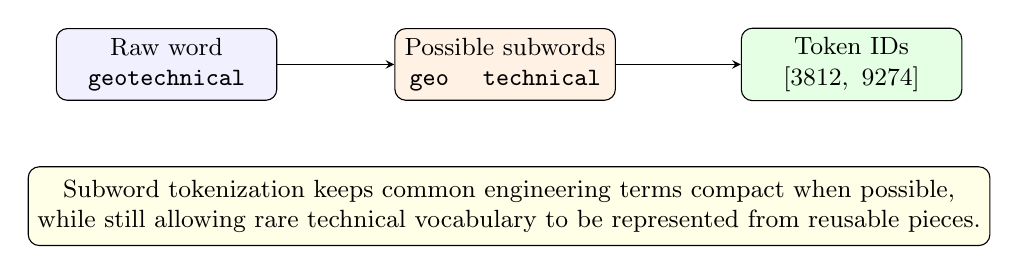
\begin{tikzpicture}[>=stealth, font=\small, x=1cm, y=1cm]
        \tikzset{box/.style={draw, rounded corners, minimum width=2.8cm, minimum height=0.8cm, align=center}}
        \node[box, fill=blue!6] (raw) at (0,0) {Raw word\\\texttt{geotechnical}};
        \node[box, fill=orange!10] (sub) at (4.3,0) {Possible subwords\\\texttt{geo} \quad \texttt{technical}};
        \node[box, fill=green!10] (ids) at (8.7,0) {Token IDs\\$[3812,\ 9274]$};
        \draw[->] (raw) -- (sub);
        \draw[->] (sub) -- (ids);

        \node[box, fill=yellow!10, minimum width=9.2cm, minimum height=1.0cm] (why) at (4.35,-1.8) {Subword tokenization keeps common engineering terms compact when possible,\\while still allowing rare technical vocabulary to be represented from reusable pieces.};
    \end{tikzpicture}
    \caption{Subword tokenization of a technical term. Modern tokenizers often break specialized vocabulary into reusable pieces before mapping those pieces to integer token IDs.}
    \label{t15fig:tokenization_schematic}
\end{figure}

\begin{ex-box}
\textbf{Why tokenization matters in engineering.} A phrase like ``ACI 318 load combination'' contains ordinary English, a code name, and a domain-specific term. Tokenization determines how efficiently the model represents that phrase. This affects cost, context-window usage, and sometimes even output quality.
\end{ex-box}

\section{From Tokens to Vectors}

\subsection{Embeddings}

Each token is mapped to a vector of real numbers, called an \textbf{embedding}. The embedding is not manually assigned. It is learned during training so that tokens appearing in similar contexts tend to acquire related vector representations.

Mathematically, if the vocabulary has size $|\mathcal{V}|$ and the embedding dimension is $d$, then the embedding table is a matrix
\begin{equation}
    E \in \mathbb{R}^{|\mathcal{V}| \times d}.
    \label{t15eq:embedding_matrix}
\end{equation}
Looking up a token returns one row of this matrix.

\begin{def-box}
\textbf{Token versus embedding.} A token is a discrete symbol. An embedding is its continuous numerical representation. Tokenization discretizes language; embeddings place that language in a vector space where similarity can be computed.
\end{def-box}

\subsection{Why High-Dimensional Spaces Matter}

Embeddings live in high-dimensional spaces, often with hundreds or thousands of coordinates. This sounds abstract, but the idea is simple. A high-dimensional vector can encode many weak signals at once: syntax, topic, tone, domain, and contextual associations.

In such spaces, tokens or passages with related meanings tend to lie near one another under a similarity measure such as cosine similarity:
\begin{equation}
    \mathrm{cos\_sim}(\mathbf{u},\mathbf{v}) = \frac{\mathbf{u}^\top \mathbf{v}}{\|\mathbf{u}\|\,\|\mathbf{v}\|}.
    \label{t15eq:cosine}
\end{equation}
This is why embedding spaces can support semantic search. A query about ``steel design loads'' may retrieve passages using related but not identical wording such as ``load combinations for structural steel members.''

\begin{figure}[ht]
    \centering
    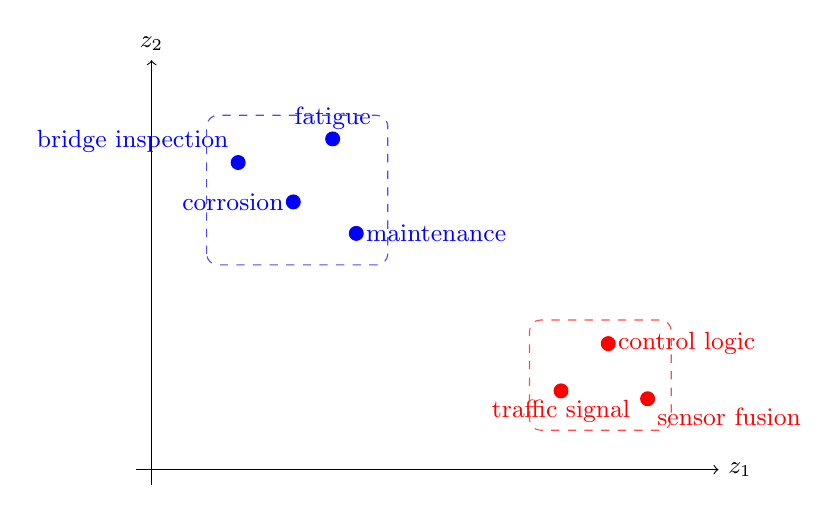
\begin{tikzpicture}[scale=1.0, every node/.style={font=\small}]
        \draw[->] (-0.2,0) -- (7.2,0) node[right] {$z_1$};
        \draw[->] (0,-0.2) -- (0,5.2) node[above] {$z_2$};

        \filldraw[blue] (1.1,3.9) circle (2.5pt) node[above left] {bridge inspection};
        \filldraw[blue] (1.8,3.4) circle (2.5pt) node[left] {corrosion};
        \filldraw[blue] (2.3,4.2) circle (2.5pt) node[above] {fatigue};
        \filldraw[blue] (2.6,3.0) circle (2.5pt) node[right] {maintenance};

        \filldraw[red] (5.2,1.0) circle (2.5pt) node[below] {traffic signal};
        \filldraw[red] (5.8,1.6) circle (2.5pt) node[right] {control logic};
        \filldraw[red] (6.3,0.9) circle (2.5pt) node[below right] {sensor fusion};

        \draw[dashed, rounded corners, blue!70] (0.7,2.6) rectangle (3.0,4.5);
        \draw[dashed, rounded corners, red!70] (4.8,0.5) rectangle (6.6,1.9);
    \end{tikzpicture}
    \caption{Low-dimensional view of an embedding space. In practice, embeddings live in hundreds or thousands of dimensions, but the same intuition applies: semantically related items tend to cluster near one another.}
    \label{t15fig:embedding_cartoon}
\end{figure}

\begin{ex-box}
\textbf{Geometric intuition.} Imagine a library in which documents are arranged not alphabetically but by meaning. Documents about bridge inspection, fatigue, corrosion, and maintenance would cluster near one another even if they use different vocabulary. An embedding space tries to create that kind of geometry numerically.
\end{ex-box}

\subsection{A Minimal Workflow View}

The front end of an LLM pipeline can be summarized as follows:

\begin{figure}[ht]
\centering
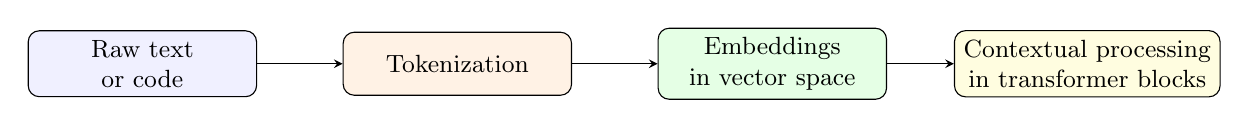
\begin{tikzpicture}[>=stealth,font=\small]
    \tikzset{box/.style={draw, rounded corners, minimum width=2.9cm, minimum height=0.8cm, align=center}}
    \node[box, fill=blue!6] (text) at (0,0) {Raw text\\or code};
    \node[box, fill=orange!10] (tok) at (4,0) {Tokenization};
    \node[box, fill=green!10] (emb) at (8,0) {Embeddings\\in vector space};
    \node[box, fill=yellow!12] (ctx) at (12,0) {Contextual processing\\in transformer blocks};
    \draw[->] (text) -- (tok);
    \draw[->] (tok) -- (emb);
    \draw[->] (emb) -- (ctx);
\end{tikzpicture}
\caption{Front-end representation pipeline for an LLM. Topic 15 focuses on the transition from raw language to token IDs to embeddings, because that representation layer makes later contextual reasoning and retrieval possible.}
\label{t15fig:minimal_pipeline}
\end{figure}

In this chapter, the main emphasis is on the first half of that pipeline: how text becomes vectors and why those vectors are useful.

\section{Sentence and Document Embeddings}

So far we have discussed token embeddings. In many engineering workflows, however, we do not want to compare single tokens. We want to compare larger chunks: sentences, paragraphs, table descriptions, code blocks, or full report sections.

The high-level strategy is to compute a representation for a larger unit of text. Conceptually, if a chunk contains token embeddings $\mathbf{e}_1,\dots,\mathbf{e}_m$, one simple aggregation idea is
\begin{equation}
    \mathbf{s} = \frac{1}{m} \sum_{i=1}^m \mathbf{e}_i,
    \label{t15eq:sentence_mean}
\end{equation}
though modern embedding models use more sophisticated contextual pooling than a simple mean.

The important teaching point is not the exact architecture. It is that an entire sentence or paragraph can also be mapped to a vector, allowing semantic comparison between chunks of text rather than only between words.

\begin{table}[ht]
    \centering
    \caption{Example chunking choices for engineering documents.}
    \begin{tabulary}{\textwidth}{L L}
        \toprule
        \textbf{Source material} & \textbf{Possible chunk} \\
        \midrule
        Design code PDF & one clause or one paragraph \\
        Structural report & one subsection or executive-summary paragraph \\
        Spreadsheet note export & one row with neighboring notes \\
        Python script & one function or one docstring-plus-function block \\
        Inspection log & one observation entry \\
        \bottomrule
    \end{tabulary}
\end{table}

Chunking matters because it determines what the retrieval system can return. If chunks are too small, meaning is fragmented. If they are too large, retrieval becomes noisy and expensive.

\section{Vector Stores and Retrieval}

Once documents, paragraphs, code blocks, or table descriptions are converted into embeddings, those vectors can be stored and searched. A \textbf{vector store} is a database or indexing system designed for this purpose.

The basic pipeline is:
\begin{enumerate}
    \item break a document collection into chunks;
    \item embed each chunk as a vector;
    \item store the vector together with metadata such as source file, page, section, and original text; and
    \item given a new query, embed the query and retrieve nearby vectors.
\end{enumerate}

This is useful because exact keyword matching is often too weak for technical work. An engineer may ask about ``serviceability limits for deflection'' while the relevant document uses a different phrase. Vector retrieval can still surface the right material because it compares meanings rather than exact strings.

\subsection{Similarity Search}

Suppose a query embedding is $\mathbf{q}$ and stored chunk embeddings are $\mathbf{v}_1,\dots,\mathbf{v}_N$. A basic retrieval score is
\begin{equation}
    s_i = \mathrm{cos\_sim}(\mathbf{q},\mathbf{v}_i),
    \qquad i=1,\dots,N,
    \label{t15eq:retrieval_score}
\end{equation}
and the system returns the top-$k$ chunks:
\begin{equation}
    \mathcal{R}_k(\mathbf{q}) = \operatorname{TopK}_{i=1,\dots,N}\; s_i.
    \label{t15eq:topk}
\end{equation}

Operational systems may use dot product, Euclidean distance, approximate nearest-neighbor indexing, reranking, or hybrid keyword-plus-vector search. But the educational core remains the same: represent the query and documents in the same vector space, then retrieve neighbors.

\subsection{Keyword Search versus Semantic Search}

It is useful to distinguish semantic retrieval from ordinary keyword retrieval. Keyword search asks whether the query words appear in the document. Semantic search asks whether the meanings are close in the embedding space. In practice, engineering systems often need both.

\begin{table}[ht]
    \centering
    \caption{Keyword search and semantic search play different roles.}
    \begin{tabulary}{\textwidth}{L L L}
        \toprule
        \textbf{Query type} & \textbf{Keyword search is strong when} & \textbf{Semantic search is strong when} \\
        \midrule
        Exact clause lookup & the exact code citation or phrase is known & wording varies across documents \\
        Prior project search & repeated terminology is consistent & similar ideas are expressed with different phrases \\
        Spreadsheet or note lookup & identifiers and labels are exact & assumptions are paraphrased in prose \\
        Research support & proper nouns and exact terms matter & concept-level similarity matters more than shared words \\
        \bottomrule
    \end{tabulary}
\end{table}

For this reason, many production systems use \textbf{hybrid retrieval}: exact matching for precision and vector similarity for semantic recall. That combination is especially natural in engineering, where code names, member labels, project IDs, and equations often require exact lookup, while design reasoning and narrative explanations benefit from semantic search.

\subsection{How Can a Sentence Be Retrieved from a Vector Store?}

This is one of the most important conceptual questions in this topic. A vector store does not literally store meaning in words. It stores numerical vectors \emph{and} references back to the original text.

In practice, each stored item looks conceptually like this:
\begin{center}
\begin{tabular}{llll}
\toprule
ID & Vector & Source metadata & Original chunk text \\
\midrule
17 & $\mathbf{v}_{17}$ & Report A, p. 42 & ``Deflection under service load shall...'' \\
18 & $\mathbf{v}_{18}$ & Report B, p. 11 & ``Load combinations for steel beams...'' \\
19 & $\mathbf{v}_{19}$ & Code note & ``Drainage layer prevents hydrostatic...'' \\
\bottomrule
\end{tabular}
\end{center}

When the query vector is close to $\mathbf{v}_{17}$, the system does not return the vector itself to the human user. It uses the stored ID and metadata to return the associated chunk text. In other words, the vector is the search key, while the original sentence or paragraph remains the human-readable payload.

\begin{figure}[ht]
    \centering
    \begin{tikzpicture}[scale=1.0, every node/.style={font=\small}]
        \draw[->] (-0.2,0) -- (7.2,0) node[right] {$z_1$};
        \draw[->] (0,-0.2) -- (0,5.2) node[above] {$z_2$};

        \filldraw[blue] (1.5,4.1) circle (2.5pt) node[above] {chunk 17};
        \filldraw[blue] (2.2,3.6) circle (2.5pt) node[left] {chunk 18};
        \filldraw[blue] (1.8,2.9) circle (2.5pt) node[left] {chunk 24};
        \filldraw[blue] (5.7,1.4) circle (2.5pt) node[right] {chunk 52};
        \filldraw[blue] (6.1,2.0) circle (2.5pt) node[right] {chunk 53};

        \filldraw[red] (1.9,3.8) circle (3pt) node[above right] {query};
        \draw[thick, red, dashed] (1.9,3.8) circle (0.7);

        \draw[->, thick, red] (1.9,3.8) -- (1.55,4.05);
        \draw[->, thick, red] (1.9,3.8) -- (2.15,3.62);
    \end{tikzpicture}
    \caption{Nearest-neighbor retrieval in an embedding space. The query is embedded into the same vector space as the stored chunks, and the nearest chunk IDs are then used to recover the original sentences or paragraphs.}
    \label{t15fig:retrieval_cartoon}
\end{figure}

\subsection{A Small Numerical Example}

Consider a simplified query and three stored chunks. Suppose the query is
\[
    q = \texttt{"serviceability limit for beam deflection"},
\]
and the cosine similarities are computed as shown in Table~\ref{t15tab:retrieval_example}.

\begin{table}[ht]
    \centering
    \caption{A toy retrieval example.}
    \label{t15tab:retrieval_example}
    \begin{tabulary}{\textwidth}{L C L}
        \toprule
        \textbf{Stored chunk} & \textbf{Cosine similarity} & \textbf{Interpretation} \\
        \midrule
        ``Deflection under service loads shall remain within specified limits.'' & 0.92 & Highly relevant \\
        ``Ultimate strength combinations control flexural resistance.'' & 0.67 & Related but not the best match \\
        ``Retaining wall drainage layers reduce pore pressure.'' & 0.18 & Largely unrelated \\
        \bottomrule
    \end{tabulary}
\end{table}

The system returns the first chunk because its vector lies nearest to the query vector under the chosen metric. The essential point is that semantic retrieval works even if the exact phrase ``beam deflection'' does not appear in the returned sentence.

\begin{alert-box}
\textbf{Important caution:} A vector store does not make an LLM correct. It only improves the chance that the model sees relevant material. The final answer can still be incomplete, misleading, or wrong if the retrieved context is poor or if the model interprets it badly.
\end{alert-box}

\subsection{Why Metadata Matters}

Metadata is the bridge back to the engineering source of truth. A vector alone is not enough. Engineers usually need to know:
\begin{itemize}
    \item which document the retrieved chunk came from,
    \item what page or section it belongs to,
    \item whether it came from a design code, internal report, spreadsheet note, or source code file, and
    \item whether the source is current, approved, or superseded.
\end{itemize}

Without metadata, a system may retrieve semantically similar text but fail to support traceability, verification, or auditability.

\begin{ex-box}
\textbf{Engineering example.} Suppose a firm has thousands of PDF reports, specifications, code excerpts, and spreadsheet notes. A vector store can index chunks from those sources so that a query such as ``find examples of retaining wall drainage design assumptions in prior projects'' retrieves semantically related passages even when the exact wording varies across projects. The useful answer is not only the retrieved text; it is also the project name, report section, and page where that text came from.
\end{ex-box}

\section{Scale and Modern LLM Training}

\subsection{Scale}

Large datasets, specialized hardware, and engineering improvements in distributed training made it possible to train models with billions of parameters. Empirically, larger models trained on more data often show smoother improvements in language tasks, coding tasks, and question answering. This observation is one reason modern AI discussions frequently emphasize scaling laws.

\subsection{What Does ``7B'' or ``70B'' Mean?}

In public discussions, the size of an LLM is often summarized by the number of \textbf{parameters}. A model described as ``7B'' has roughly seven billion trainable weights; ``70B'' means roughly seventy billion; and ``1T'' means roughly one trillion. This shorthand is imperfect, but it remains the most common public indicator of model scale.

Students should interpret this number carefully. Parameter count is not the same as intelligence, and it is not the same as memory in the usual human sense. It is better to think of parameters as the adjustable coefficients that store the model's learned statistical structure. During training, those coefficients are repeatedly updated; during inference, they are fixed.

For a simple example, the embedding matrix alone already contains
\begin{equation}
    |\mathcal{V}|\times d
    \label{t15eq:embedding_param_count}
\end{equation}
parameters. If $|\mathcal{V}|\approx 50{,}000$ and $d=12{,}288$, then the embedding layer by itself contains roughly
\[
    50{,}000\times 12{,}288 \approx 6.1\times 10^8
\]
parameters, that is, hundreds of millions of weights before counting the attention blocks and feedforward layers.

\begin{table}[ht]
    \centering
    \caption{Representative public shorthand for model size.}
    \label{t15tab:model_scale}
    \begin{tabular}{lcc}
        \toprule
        \textbf{Model family example} & \textbf{Parameter count} & \textbf{Public shorthand} \\
        \midrule
        Small open model & $7\times 10^9$ & 7B \\
        Larger open model & $70\times 10^9$ & 70B \\
        GPT-3 class & $175\times 10^9$ & 175B \\
        Frontier-scale model & $>10^{12}$ & $>$1T \\
        \bottomrule
    \end{tabular}
\end{table}

\begin{def-box}
\textbf{Working interpretation of parameter count.} The number of parameters is a rough proxy for model capacity, engineering cost, and deployment complexity. It is useful, but it should always be interpreted together with training data quality, compute budget, architecture, and post-training.
\end{def-box}

\subsection{Why Training Requires GPU Clusters}

Training a modern LLM is far more demanding than running it for inference. During training, the system must repeatedly perform forward passes, backpropagation, and optimizer updates over enormous matrices. This is exactly the type of workload for which GPUs are well suited: large parallel tensor operations.

The need for GPU clusters follows from several pressures acting at once:
\begin{itemize}
    \item the model weights themselves may occupy many gigabytes or terabytes;
    \item activations from forward passes must often be stored for backpropagation;
    \item optimizer states add substantial extra memory beyond the raw weights; and
    \item the training corpus may contain trillions of tokens, making wall-clock time a major concern.
\end{itemize}

For this reason, modern LLM training is distributed across many accelerators. In rough terms, one must split the work across devices because a single GPU often cannot hold the full training state efficiently, and even when it can, the training time would be impractically long. The engineering challenge is therefore not just machine learning; it is also systems design, networking, storage, and parallel computing.

\subsection{Mixture of Experts}

As models grew, researchers also explored \textbf{mixture-of-experts} (MoE) designs. In an MoE model, only part of the network is activated for a given token or input. One can think of this as routing work to specialized sub-networks rather than forcing every parameter to process every token. A high-level expression is
\begin{equation}
    y = \sum_{i=1}^M g_i(x)\,E_i(x),
    \label{t15eq:moe}
\end{equation}
where $E_i$ denotes expert $i$ and $g_i(x)$ is a gating weight or routing score.

The motivation is practical: MoE can increase model capacity without increasing computation proportionally at every step. This is one reason some state-of-the-art systems combine dense transformer blocks with sparse expert routing.

\subsection{Training Is More Than Pretraining}

Students often hear that LLMs are trained by ``predicting the next token,'' which is true but incomplete. Modern frontier systems usually go through several stages:
\begin{enumerate}
    \item \textbf{Pretraining:} learn general language patterns from very large text and code corpora;
    \item \textbf{Continued or domain-adaptive training:} sometimes extend training on more specialized data;
    \item \textbf{Instruction tuning / supervised fine-tuning:} train the model to follow tasks and response formats more reliably; and
    \item \textbf{Preference or reinforcement-based post-training:} shape behavior according to human or programmatic feedback.
\end{enumerate}

This layered pipeline matters because the model students interact with in practice is rarely a raw pretrained model. It is usually a \emph{post-trained assistant}, meaning that it has been further shaped for helpfulness, safety, formatting, or task behavior.

\subsection{Fine-Tuning, Customization, and Alignment}

Once a base model exists, there are several ways to customize it. The most direct is supervised fine-tuning (SFT), where the model is trained on prompt-response pairs:
\begin{equation}
    \mathcal{L}_{\mathrm{SFT}}(\theta)
    = -\sum_{(x,y)\in\mathcal{D}} \log P_\theta(y\mid x).
    \label{t15eq:sft}
\end{equation}

This is effective when high-quality demonstrations are available. However, many desired behaviors are easier to express as preferences than as one ``correct'' answer. That motivates preference learning. In a classical RLHF pipeline, humans compare model outputs, a reward model is trained on those comparisons, and the policy model is then optimized to improve reward while not drifting too far from a reference model.

An influential simplification is \textbf{direct preference optimization} (DPO), which uses preferred and dispreferred response pairs directly. The exact derivation belongs to a later topic, but the intuition is simple: increase the relative probability of the preferred response while staying anchored to the original model.

At a practical level, students should remember the distinction:
\begin{itemize}
    \item \textbf{SFT} teaches the model from demonstrations;
    \item \textbf{RLHF} teaches the model from learned reward signals based on feedback; and
    \item \textbf{DPO and related methods} teach from preference pairs more directly, often with lower engineering complexity.
\end{itemize}

Another important idea is \textbf{parameter-efficient fine-tuning}. Methods such as LoRA update only small adapter-like components rather than all model weights. This matters in practice because organizations often want customization without the cost of retraining a full frontier model.

\begin{def-box}
\textbf{Working definition.} A \textbf{foundation model} is a large model trained on broad data so that the same base system can support many downstream tasks. An LLM is a foundation model specialized around language and language-like sequences such as text and code.
\end{def-box}

\begin{figure}[ht]
    \centering
    % natural width ≈ 17.2 cm
    % scale = target_width / 17.2
    \def\archscale{0.85}
    \begin{tikzpicture}[
        >=stealth,
        font=\small,
        x=1cm, y=1cm,
        scale=\archscale,
        transform shape
    ]
        \tikzset{
            block/.style={draw, rounded corners, minimum width=4.3cm, minimum height=0.9cm, align=center},
            side/.style={draw, rounded corners, minimum width=2.5cm, minimum height=0.8cm, align=center}
        }

        \node[side, fill=blue!6] (tokens) at (0,0) {Prompt tokens};
        \node[block, fill=orange!12] (embed) at (5.2,0)   {Token embeddings + positional information};
        \node[block, fill=green!10]  (attn1) at (5.2,-2.0) {Masked self-attention};
        \node[block, fill=green!10]  (ffn1)  at (5.2,-3.6) {Feedforward layer + residual path};
        \node[block, fill=green!10]  (attn2) at (5.2,-5.4) {Repeat many decoder blocks};
        \node[side, fill=yellow!12] (head) at (11.0,-2.7) {Linear layer +\\next-token probabilities};
        \node[side, fill=red!8]     (out)  at (15.0,-2.7) {Predicted next token};
        \draw[->] (tokens) -- (embed);
        \draw[->] (embed) -- (attn1);
        \draw[->] (attn1) -- (ffn1);
        \draw[->] (ffn1) -- (attn2);
        \draw[->] (attn2.east) to[out=0,in=180] (head.west);
        \draw[->] (head) -- (out);
        \draw[dashed,->] (out.south) |- ++(0,-1.4) -| (tokens.south);
    \end{tikzpicture}
    \caption{Decoder-only transformer pipeline used in GPT-style language models. Prompt tokens are embedded, processed through repeated masked-attention blocks, and converted into next-token probabilities.}
    \label{t15fig:transformer_architecture}
\end{figure}
Figure~\ref{t15fig:transformer_architecture} emphasizes an important point for this course: many well-known transformer diagrams were developed for translation, but the GPT family that dominates modern text generation is typically decoder-only and autoregressive.

\section{Generation Limits: Hallucination and Reliability}

No introductory chapter on LLMs is complete without discussing hallucination. In qualitative terms, a hallucination occurs when the model produces content that is fluent and plausible but unsupported, incorrect, fabricated, or overconfident relative to the available evidence.

Hallucination should not be understood as a mysterious malfunction. It follows from the nature of probabilistic generation. The model is optimized to continue a sequence with likely text, not to guarantee truth in the strict engineering sense. If the context is weak, ambiguous, or missing a needed fact, the model may still generate a smooth continuation.

\subsection{Why Hallucinations Occur}

Several mechanisms contribute:
\begin{itemize}
    \item \textbf{Probabilistic next-token generation:} the model predicts likely continuations, not verified facts;
    \item \textbf{Incomplete context:} the needed source may not be in the prompt or retrieval set;
    \item \textbf{Post-training pressure:} models tuned to be helpful may answer even when uncertainty is high;
    \item \textbf{Distribution shift:} specialized technical questions may lie outside the strongest regions of training data; and
    \item \textbf{Decoding choices:} sampling settings can make unlikely tokens more or less likely to appear.
\end{itemize}

This explains a common engineering observation: a model may sound very confident exactly when it should instead say ``I do not know'' or ``I need the source document.''

\subsection{Temperature and Output Reliability}

During generation, logits are converted into probabilities. A common decoding control is \textbf{temperature scaling}:
\begin{equation}
    P_T(v) \propto \exp\!\left(\frac{\log P(v)}{T}\right),
    \label{t15eq:temperature}
\end{equation}
where $T$ is the temperature. Lower temperature sharpens the distribution, making the model more likely to choose the most probable next token. Higher temperature flattens the distribution, allowing lower-probability tokens to be sampled more often.

This does \emph{not} change what the model has learned. It changes how aggressively the generation procedure explores alternatives. For factual or technical tasks, lower temperatures often reduce gratuitous variation and can reduce some forms of hallucination. For creative tasks, higher temperatures can be useful. But low temperature is not a guarantee of truth: if the highest-probability continuation is wrong, greedy decoding may still be wrong.

\begin{table}[ht]
    \centering
    \caption{Qualitative effect of temperature in generation.}
    \label{t15tab:temperature}
    \begin{tabulary}{\textwidth}{L L L}
        \toprule
        \textbf{Temperature range} & \textbf{Typical behavior} & \textbf{Use case} \\
        \midrule
        Low ($0$--$0.3$) & focused, repetitive, lower variance & coding, extraction, factual QA \\
        Medium ($0.4$--$0.7$) & balanced fluency and variety & analysis, summarization, normal chat \\
        High ($0.8+$) & diverse, exploratory, higher variance & brainstorming, creative writing \\
        \bottomrule
    \end{tabulary}
\end{table}

\begin{alert-box}
\textbf{Important limitation:} Lower temperature may reduce some hallucinations, but it does not solve the core problem of missing knowledge, weak retrieval, or miscalibration. A deterministic wrong answer is still wrong.
\end{alert-box}

\subsection{How Engineers Should Respond to Hallucination}

The practical lesson is not ``never use LLMs.'' It is ``use them with the right control structure.'' In engineering settings, hallucination risk should be reduced by:
\begin{itemize}
    \item grounding answers in retrieved documents or cited standards;
    \item using lower-variance decoding for factual tasks;
    \item asking for sources, assumptions, and intermediate checks;
    \item treating outputs as drafts or candidates rather than final truth; and
    \item keeping a human reviewer in the loop for consequential decisions.
\end{itemize}

\section{Putting the Pieces Together}

We can now summarize the document-retrieval pipeline that connects LLMs to engineering knowledge work:

\begin{enumerate}
    \item technical documents are split into chunks;
    \item each chunk is converted into an embedding vector;
    \item vectors and metadata are stored in a searchable index;
    \item a user query is embedded into the same vector space;
    \item the system finds the nearest stored vectors; and
    \item the original text chunks are returned, optionally to be passed into an LLM for synthesis.
\end{enumerate}

This is why LLM-era systems are powerful in engineering. They operate on the same document universe that engineers already inhabit. The vector layer is what makes meaning-based retrieval practical, while post-training and decoding choices shape how the model behaves once that information is available.

\section{What This Chapter Covers and What Comes Next}

This chapter focused on motivation and representation. We began with the engineering need: technical work is dominated by documents and language-like artifacts. We then reviewed why NLP was historically difficult, why transformers and GPT-style pretraining changed the field, how model size and GPU-based training entered the picture, and why tokenization and embeddings are central to modern language systems. We also introduced post-training ideas such as supervised fine-tuning, preference optimization, and alignment at a conceptual level. Finally, we introduced vector stores as a practical bridge from language models to document-centered engineering workflows, including the key question of how a human-readable sentence is retrieved from numerical vectors and why hallucination remains a practical limitation.

Topic 16 will build on this foundation. There we will examine the mainstream internal architectures of modern LLM systems in more detail and then turn to the larger opportunity space: prompting workflows, knowledge engineering, agentic AI, and coding or planning assistants. That discussion naturally leads to Topic 17, where the central question becomes human-in-the-loop engineering: how people should work with these systems, where the risks lie, and why ethics and accountability remain essential.

\end{document}
